% !TEX encoding = UTF-8 Unicode
% ÄÖÜ ß äöü

The aim of this project was to design an interactive environment on a tablet computer 
that allows the user to learn simple facts about the formalism of propositional logic 
and standard transformations of Boolean functions. 
The environment is meant to be self-explanatory. 

The core of this concept builds on tutorials with exercises 
and a playground where the learned knowledge can be used in different modes. 
A glossary of terms and a formula calculator (BoolTool) to check formulas will support the user in their learning.

\section{Tutorials}

Ny$\bar{a}$ya for iPad covers syntax and semantics of propositional logic, but not natural deduction. 
It introduces normal forms and the representation of boolean functions
as truth tables and binary decision diagrams. 

The structure of the tutorials and the content of the exercises are heavily based on the according sections of the book  
{\em Logic in Computer Science} \cite{Huth:2004:LCS:975331} by M.~Huth and M.~Ryan.
Additional content is taken from the lecture {\em Logic} \cite{Middeldorp:2012:LICS} by {A. Middeldorp}

Every tutorial includes a teaching part with examples (simple html files in utf8 encoding) and interactive challenges, 
where the user gets immediate feedback. Every interactive part will present some instructions to master the challenge.

\subsection{Introduction}

The first three tutorials give an overview to modeling, 
i.e. the translation from sentences of natural language to more formal sentences. 
The content and configuration of the comprehensive questions are stored in xml-files in utf8-encoding. 

The content is written into  a simple property list “QA124.plist” \tabref{tab:QA123} 
with an array (starts at line 2) 
of arrays that include sentences and sample solutions (the first exercise-array starts at line 3). 
The first string is the sample sentence (line 4), 
and the following entries are the solutions for different exercises. 

The tutorials has their own configuration files “NyTuTester101.plist” \tabref{tab:PLIST101},
 “NyTuTester111.plist” and  “NyTuTester121.plist”, with a dictionary that
 describes the task and defines the index of the sample solution.


\begin{table}[htdp]
\begin{center}
\begin{lstlisting}[mathescape]
<?xml version="1.0" encoding="UTF-8"?>
<!DOCTYPE plist PUBLIC "-//Apple//DTD PLIST 1.0//EN" "http://www.apple.com/DTDs/PropertyList-1.0.dtd">
<plist version="1.0">
	<array>
		<array> 
			<string>If the barmoter falls, then it will rain or it will snow.</string>
			<string>if p then q or r</string>
			<string>the barometer falls; it will rains; it will snow</string>
			<string>p $\rightarrow$ q $\vee$ r</string>
		</array>
		<array>
			<string>sample sentence …
			$\square$
		$\square$
	$\square$
</plist>
\end{lstlisting}
\caption{Content file with sentences and solutions}
\end{center}
\label{tab:QA123}
\end{table}%

\begin{table}[htdp]
\begin{center}
\begin{lstlisting}[mathescape]
<?xml version="1.0" encoding="UTF-8"?>
<!DOCTYPE plist PUBLIC "-//Apple//DTD PLIST 1.0//EN" "http://www.apple.com/DTDs/PropertyList-1.0.dtd">
<plist version="1.0">
<dict>
 <key>keyLabelText</key>
 <string>Guess the structure of composite sentences</string>
 <key>inputLabelText</key>
 <string>Use only “if”, “then”, “and”, “or“, “not”, “p”, “q”, “r”.</string>
 <key>valueLabelText</key>
 <string>Sample solution (you may have found an other correct epression)</string>
 <key>questionsFile</key>
 <string>QA123</string>
 <key>answerIndex</key>
 <integer>1</integer>
</dict>
\end{lstlisting}
\caption{Configuration file with comprehension question}
\end{center}
\label{tab:PLIST101}
\end{table}%


\begin{verbatim}
\end{verbatim}

\subsubsection{Motivation – the composite structure of sentences}

The aim of logic in general is to reason about situations.\cite{Huth:2004:LCS:975331} 
The common structure of two composite sentences in natural language 
is reduced to “If p and not q, then r. Not r. p. Therefore, q“. 
If the reasoning is correct, the user can it use in both situations.
In the interactive part the user has to guess the structure of composite sentences. 

\subsubsection{Propositions – declarative sentences}

The concept of propositions – declarative sentences – 
as indivisible building blocks of propositional logic 
is explained in more detail. Some counterexamples are presented 
and the ambiguity of natural language is demonstrated.
The user has to find the propositions in composite sentences. 

\subsubsection{Symbols – emphasize the structure}

The symbols to replace “if then”, “not”, “and” and “or” are introduced. 
Now the user should transform the sentences from the first tutorial into pure propositional formulas. 
The content will be generated by the app and the user's solution will be checked without tolerance.

\subsubsection{Limits}

Not every situation can be transformed into a formula in propositional logic. 
This tutorial has no interactive part.

\subsection{Syntax}

After the informal introduction into the atoms and connectives of propositional logic, 
the formal aspects of propositional logic will be introduced to the user.

\subsubsection{Well formed formulas}

The concept of well formed formulas is explained. 
The user has to build simple well formed formulas: 
“a conjcuntion”, “an disjunction of an negation”, “a negation of an implication” and so on.
They have to use parenthesis.

\subsubsection{Conventions for your convenience}

Precedence of connective is introduced. 
The user has to rewrite formulas 
to save some parenthesis.

\subsubsection{Subformulas}

Subformulas (starting from atoms) are use to build bigger formulas. Big formulas are build from many sub formulas.
The user have to find all sub formulas of simple composite formulas.

\subsubsection{Syntax Trees}

This tutorial explains how to draw an syntax tree (starting with atoms)
The user has to draw the syntax tree of simple formulas.

\subsubsection{Additional symbols – Top and Bottom}

The tutorial introduces top and bottom  
as abbreviations of conjunctions and disjunctions 
of formulas with their negation (tautologies and contradictions)

\subsubsection{Simplifying formulas}

The tutorial teaches the simplifying of conjunctions and disjunctions with top and bottom.

\subsection{Semantics}

After the introduction of well formed formulas the meaning of logical connectives is defined.

\subsubsection{Truth assignments and valuation of formulas}

The user has to guess or calculate the evaluation of a given formula with a given truth assignment of the atoms of the formula.

\subsubsection{Truth tables}

The user has to fill in complete truth tables.

\subsubsection{Entailment and Equivalence}



\subsubsection{Satisfiability, Tautologies and Contradictions}

content is missing

\subsection{Normal Forms}

\subsubsection{Implication Free Form}

content is missing

\subsubsection{Negation Normal Form}

content is missing

\subsubsection{Conjunctive Normal Form}

content is missing

\subsubsection{Disjunctive Normal Form}

content is missing

\subsubsection{Algorithms combined}

content is missing

\subsection{Binary Decision Diagrams}

content is missing


%Propositional formulae are build from atoms and connectives.

%\begin{itemize}
%
%\item Write a formula with given symbols.
%
%\item Write a disjunction/implication/negation/conjunction with given symbols.
%
%\end{itemize}

%\subsection{Sub formulae}

%Every formula is build from sub formulae.

%\begin{itemize}
%
%\item Find all sub formulae of given formula. (Figure~\ref{tutfig:findallsubformulae}~und~\ref{impfig:findallsubformulae})
%
%\end{itemize}
%
%\begin{figure}[htdp]
%\caption{Find all sub formulae}
%\begin{center}
%\begin{tabular}{|p{0.5cm}|p{0.5cm}|p{1cm}|p{1.5cm}|p{2.5cm}|c|}
%\hline
% &  &  &  & & $\Phi=(\neg (p \rightarrow q) \wedge q) \vee q $\\
%\hline
%\end{tabular}
%\end{center}
%\label{tutfig:findallsubformulae}
%\end{figure}

%\subsection{Syntax tree}

%A syntax trees is just an other visual representation of a propositional formula. 
%
%\begin{itemize}
%
%\item Build syntax tree for given formula. (Figure~\ref{tutfig:FormulaToTree})
%
%\item Write formula for given syntax tree. (Figure~\ref{tutfig:TreeToFormua})
%
%\end{itemize}

%\subsection{Syntax Conventions}

%\begin{itemize}
%\item Remove parenthesis
%\item Add parenthesis.
%\end{itemize}

%\subsection{Semantics: Valuation and Extension}

%Valuation (truth assignment) is mapping from atom to truth values.
%
%\begin{itemize}
%\item Determine truth value for given formula and given truth assignment. (Figure~\ref{tutfig:computeextension}~und~\ref{impfig:computeextension})
%\end{itemize}
%
%\begin{figure}[htdp]
%\caption{Compute extension of given truth assignment.}
%\begin{center}
%\begin{tabular}{|c|c|c|c|c|c|}
%\hline
%p & q & $p\rightarrow q$ & $\neg (p\rightarrow q$) & $\neg (p\rightarrow q) \wedge q$& $\Phi=(\neg (p \rightarrow q) \wedge q) \vee q $\\
%\hline \hline
%T&F&&&&\\
%\hline
%\end{tabular}
%\end{center}
%\label{tutfig:computeextension}
%\end{figure}

%\subsection{Semantics: Truth Tables}

%A truth table contains all possible truth assignments for a formula.
%
%\begin{itemize}
%\item Fill truth tables. (Figure~\ref{tutfig:filltruthtable}~und~\ref{impfig:filltruthtable})
%\end{itemize}
%
%\begin{figure}[htdp]
%\caption{Fill truth table for given formula}
%\begin{center}
%\begin{tabular}{|c|c|c|c|c|c|}
%\hline
%p & q & $p\rightarrow q$ & $\neg (p\rightarrow q$) & $\neg (p\rightarrow q) \wedge q$& $\Phi=(\neg (p \rightarrow q) \wedge q) \vee q $\\
%\hline\hline
%T&T&&&&\\
%T&&&&&\\
%F&&&&&\\
%&&&&&\\
%\hline
%\end{tabular}
%\end{center}
%\label{tutfig:filltruthtable}
%\end{figure}%


%\subsection{Semantic entailment}

%\begin{itemize}
%\item Check semantic entailment (Figure~\ref{tutfig:CheckSemanticEntailment})
%\end{itemize}
%
%\begin{figure}[htdp]
%\caption{Check semantic entailment.}
%\begin{center}
%\begin{tabular}{|c|c||c|c|c|c|c|c|c|c|c|c|}
%\hline
%&  & $\Phi$ & $\Psi$ & $\Xi$ 
%& $\Phi,\Psi \vDash \Xi$ 
%& $\Phi,\Xi \vDash \Psi$ 
%& $\Psi,\Xi \vDash \Phi$ 
%& $L,R \vDash R$\\
%L & R & $\neg(L \vee R)$ & $\neg L \vee \neg R$ & $\neg L \wedge \neg R$ & $\square$ & $\square$& $\square$& $\square$\\
%\hline\hline
%T&T&&& &$\square$ & $\square$& $\square$& $\square$\\
%T&F&&&& $\square$ & $\square$& $\square$& $\square$\\
%F&T&&&& $\square$ & $\square$& $\square$& $\square$\\
%T&F&&&& $\square$ & $\square$& $\square$& $\square$\\
%\hline
%\end{tabular}
%\end{center}
%\label{tutfig:CheckSemanticEntailment}
%\end{figure}%


%\subsection{Semantic equivalence}

%\begin{itemize}
%\item Check semantic entailment (Figure~\ref{tutfig:CheckSemanticEquivalence})
%\end{itemize}
%
%\begin{figure}[htdp]
%\caption{Check semantic equivalence.}
%\begin{center}
%\begin{tabular}{|c|c|c|c|c|c|c|c|c|}
%\hline
%&  & $\Phi$ & $\Psi$ & $\Xi$& $\Phi \equiv \Psi$ & $\Phi \equiv \Xi$ & $\Xi \equiv \Psi$ & $L \equiv R$ \\
%L & R & $\neg(L \vee R)$ & $\neg L \vee \neg R$ & $\neg L \wedge \neg R$ & $\square$ & $\square$& $\square$& $\square$\\
%\hline\hline
%T&T&&& &$\square$ & $\square$& $\square$& $\square$\\
%T&F&&&& $\square$ & $\square$& $\square$& $\square$\\
%F&T&&&& $\square$ & $\square$& $\square$& $\square$\\
%T&F&&&& $\square$ & $\square$& $\square$& $\square$\\
%\hline
%\end{tabular}
%\end{center}
%\label{tutfig:CheckSemanticEquivalence}
%\end{figure}%
%


%\subsection{Equivalence transformations}

%$\neg (L \vee R) \equiv \neg L \wedge \neg R$ (Figure~\ref{tutfig:nnf_disjunction})
%
%\begin{figure}[htdp]
%\caption{$\neg (L \vee R) \equiv \neg L \wedge \neg R$}
%\begin{center}
%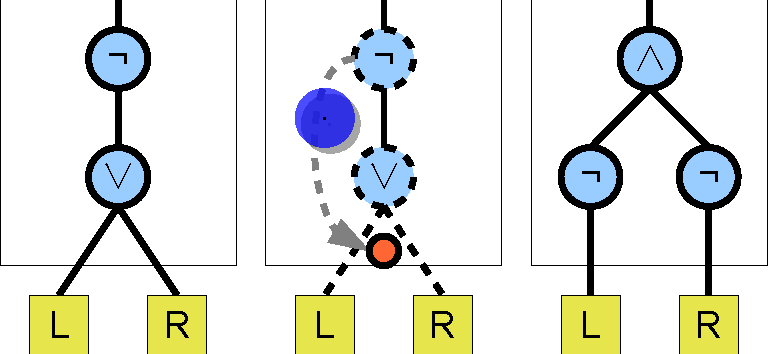
\includegraphics[scale=0.9]{drawings/nnf_disjunction.pdf}
%\end{center}
%\label{tutfig:nnf_disjunction}
%\end{figure}%
%
%\subsection{Validity and Satifiability}
%\subsection{Conjunctive Normal Form}
%
%\begin{enumerate}
%\item eleminate implications
%\item push negations towards atoms
%\item distribute disjunction over conjunction
%\end{enumerate}

%\subsection{Boolean functions}

%\subsection{Binary decision diagram}

%\subsection{Reduced BDD}

%\begin{itemize}
%\item {remove duplicate terminals} (Figure~\ref{tutfig:bdd_remove_duplicate_terminals})
%\item {remove redundant tests}
%\item {remove duplicate non-terminals}
%\end {itemize}
%
%\begin{figure}[htdp]
%\caption{Remove duplicate terminals}
%\begin{center}
%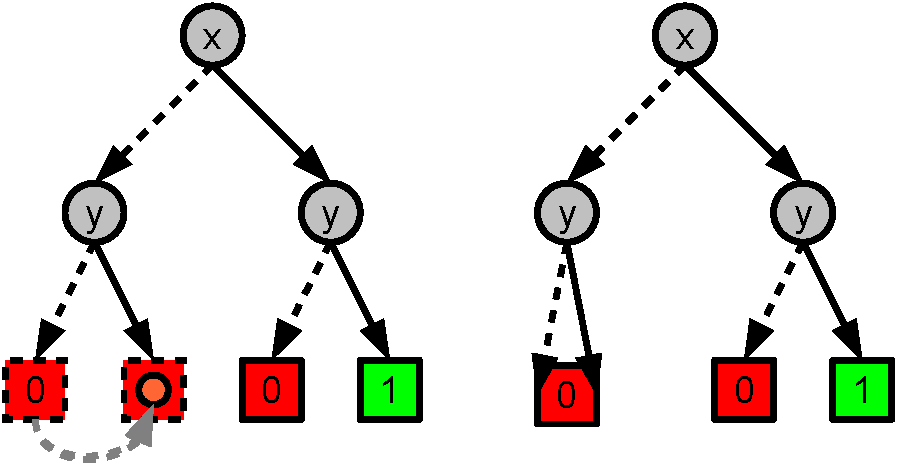
\includegraphics[scale=0.9]{drawings/bdd_remove_duplicate_terminals.pdf}
%\end{center}
%\label{tutfig:bdd_remove_duplicate_terminals}
%\end{figure}%

%\subsection{order algorithm}

%\subsection{reduce algorithm}

%\subsection{restrict algorithm}

%\subsection{shannon expansion}

%\subsection{apply algorithm}

\section{Playgrounds}

content is missing

\subsection{Create formulas by syntax tree}

content is missing

\subsubsection{Find sub formulas by syntax tree}

content is missing

\subsection{Perform equivalence transformations on the syntax tree}

content is missing

\subsubsection{Substitute implications}

content is missing

\subsubsection{Distribute negation over con- and disjunctions}

content is missing

\subsubsection{Remove double negations}

content is missing

\subsubsection{Distribute conjunctions over disjunctions and vice versa}

content is missing

\subsubsection{Substitute Contradictions and Tautologies}

content is missing

\section{Glossary}

content is missing

\section{BoolTool}

Of course the interactive environment should contain the functionality of the \href{web fronted} of BoolTool.
Some additions should be added for comfort.

\subsection{Input}

As minimum the embedded BoolTool must support the small latin letters as identifiers for atoms, 
“T” and “F” as names for top and bottom, and the symbols
“\verb#!&|+>^#” as connectives, because these symbols can be found on almost every keyboard.
In environments with native utf8-strings it is is desirable that standard symbols of propositional logic
“$ \neg \vee \wedge \rightarrow $”are accepted too, 
so the user can copy the output and paste it into the input. 
This enables the local persisting of formulas in standard representation of boolean functions.

\begin{table}[htdp]
\begin{center}%\begin{lstlisting}[mathescape] 

$\top | \perp 
| \neg | !
| \wedge | \&
| {\setminus}| | {\setminus}+
| \veebar | \oplus | \textasciicircum
| = | <> | \leftrightarrow 
| > | \rightarrow | \models
| ( | ) | , | ; 
| {\setminus}w+$ %\end{lstlisting}
\caption{Regular expresson for a lexxer to build a more flexible parser}
\end{center}
\label{tab:REGEX}
\end{table}%

\begin{table}[htdp]
\begin{center}
\begin{tabular}{l|c|c|c|cc|c|c|c|c|c|c|c|}
Name	& NOT		& AND		& OR		&  IMPLIES \\
ASCII 	& ! 			& \& \quad .	& |  \quad +			&> 	\\
Symbol  	& $\neg$		& $\wedge$	& {$\vee$}		&$\rightarrow$ \\ 
UTF-8	& C2 AC		& E2 88 A7	& {E2 88 A8}	&E2 86 92\\
Unicode	& U+00AC 	& U+2227		& {U+2228}	&U+2192\\
HTML	& \&not;		& \&and;		& \&or;		& \&rarr; 
\end{tabular}
\caption{basic connectives in ascii, utf-8, unicode and html}
\end{center}
\label{tab:BASICSYMBOLS}
\end{table}%

\begin{table}[htdp]
\begin{center}
\begin{tabular}{c|c|cc|cccccccccc}
TOP			& BOTTOM	& XOR & EOR		& IFF\\	
T \quad 1	& F  \quad 0	& \multicolumn{2}{c|}{\textasciicircum} 	& <> \\
$\top$		& $\perp$		& $\veebar$ 	&$\oplus$   			&$ \leftrightarrow$\\
E2 8A A4	& E2 8A A5	& E2 8A BB	& E2 8A 95			&E2 86 94\\
U+22A4		& U+22A5		& U+22BB	& U+2295				&U+2194\\
T			& F			&			& \&oplus;				& \&harr;
\end{tabular}
\caption{additional connectives in ascii, utf-8, unicode and html}
\end{center}
\label{tab:ADDITIONALSYMBOLS}
\end{table}%

% ⊨|⊤|⊥|¬|!|∧|&|\\.|∨|\\+|\\||=|↔|<>|→|>|⊻|⊕|\\^|\\(|\\)|,|;|\\w+

\subsection{Output}

BoolToll calculates and displays a bundle of representations of user's input. 


